\subsection{Описание алгоритма калибровки гирлянды}
\label{sec:develop:algorithm}

При использовании гирлянды пользователь может повесить ее каким угодно образом. Однако при этом часть анимаций, которые расчитаны на конкретное расположение лампочек друг от друга, будут воспроизводится некорректно, представляя из себя мешанину из цветов. Алгоритм калибровки призван устранить данный недостаток анимаций. Пользователь с помощью камеры снимает небольшую анимацию на гирлянде, а потом алгоритм обрабатывает данные снимки и понимает расположение лампочек относительно друг друга.

\subsubsection{} Анимация калибровки
\label{sec:develop:algorithm:animation}

Анимация калибровки представляет собой последовательность из трех цветов (красный, синий и зеленый) для каждой лампочки. Ее суть заключается в том, что каждой лампочке задают определенную последовательность из трех цветов (адреса представляются в троичной системе исчисления). Последовательности при каждой калибровке генерируются заново, чтобы исключить проблему, когда рядом лежащие лампы горят одним цветом, что может привести к наслоению их друг на друга при обработке изображения. Пример изображен на рисунке~\ref{fig:develop:algorithm:animation}.

Шаги анимации:
\begin{itemize}
	\item все лампочки горят синим цветом~-- нужно, чтобы алгоритм понял, что анимация началась;
	\item все лампочки гаснут~-- алгоритм использует прошлый кадр с синими лампами и этот кадр, чтобы вычленить из всего изображения место, где будут находится лампы, отфильтровав все остальные предметы с синим, красным или зеленым цветом;
	\item последовательности цветов~-- алгоритм анимирует гирлянду в трех цветах. Количество цветов в последовательности вычисляется как $\lfloor\log_3 a\rfloor$, где $a$~-- количество лампочек в гирлянде.
\end{itemize}

~
\begin{figure}[H]
\centering
	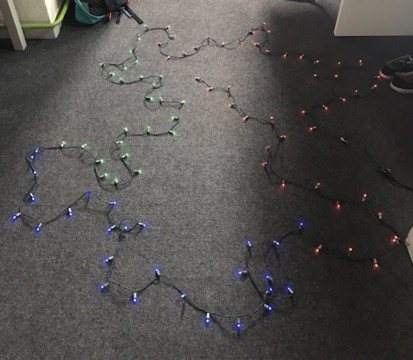
\includegraphics[scale=0.8]{figures/calibration_animation.jpg}
	\caption{Пример кадра анимации}
	\label{fig:develop:algorithm:animation}
\end{figure}

\subsubsection{} Ядро алгоритма
\label{sec:develop:algorithm:core}

База алгоритма основывается на распознании цвета пикселей изображений и на Connected-Component Labeling алгоритме. Его суть состоит в группировке одинаковых пикселей с помощью алгоритма поиска в глубину. Так как этот алгоритм предназначен для работы с изображениями только двух цветов, то нам надо превратить изображение, снятое с камеры телефона, в черно-белое. Использовать черно-белое изображение для распознания трех цветов одновременно не представляется возможным, поэтому для начала мы формируем три изображения для каждого из цветов отдельно, переводя изображение в черно-белое, где белым выделен нужный нам цвет (Рисунок~\ref{fig:develop:algorithm:colorFinding}).

~
\begin{figure}[H]
\centering
	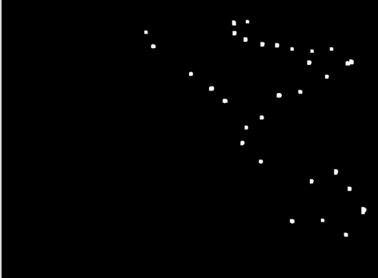
\includegraphics[scale=0.8]{figures/calibration_findedColor.jpg}
	\caption{Пример найденного цвета в кадре}
	\label{fig:develop:algorithm:colorFinding}
\end{figure}

Изображение может быть некачественным, поскольку оно сжимается для лучшей скорости работы; также еще стоит учитывать покачивания при съемке, засвет от других источников и тд. Следовательно, лампочка скорее всего будет состоять не из одной группы лежащих рядом пикселей, а из нескольких (Рисунок~\ref{fig:develop:algorithm:toBlackWhite}). Для этого применяется размытие по Гауссу вместе с фильтром по яркости (Рисунок~\ref{fig:develop:algorithm:blurring}). Далее находим группы из белых пикселей с помощью описанного выше CCL алгоритма (каждая группа - лампочка определенного цвета). При обработке всех кадров получаем последовательность из цветов с похожими координатами, так как это скорее всего одна и таже лампа, то группируем их в последовательность. Далее сопоставляем последовательность с уже заранее сгенерированными и находим адрес лампочки (Рисунок~\ref{fig:develop:algorithm:grouping}).

~
\begin{figure}[H]
\centering
	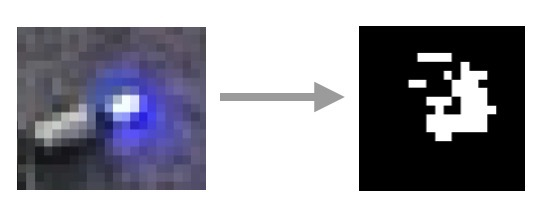
\includegraphics[scale=0.5]{figures/calibration_toBlackWhite.jpg}
	\caption{Первоначальное распознание цвета}
	\label{fig:develop:algorithm:toBlackWhite}
\end{figure}

~
\begin{figure}[H]
\centering
	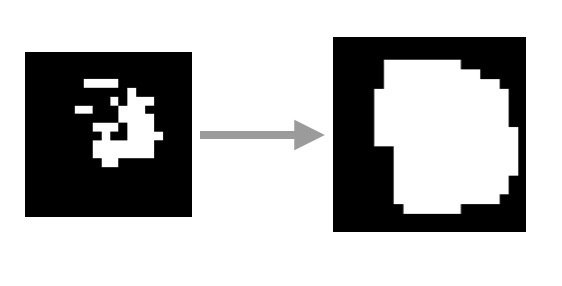
\includegraphics[scale=0.5]{figures/calibration_blurring.jpg}
	\caption{Распознание цвета после размытия}
	\label{fig:develop:algorithm:blurring}
\end{figure}

~
\begin{figure}[H]
\centering
	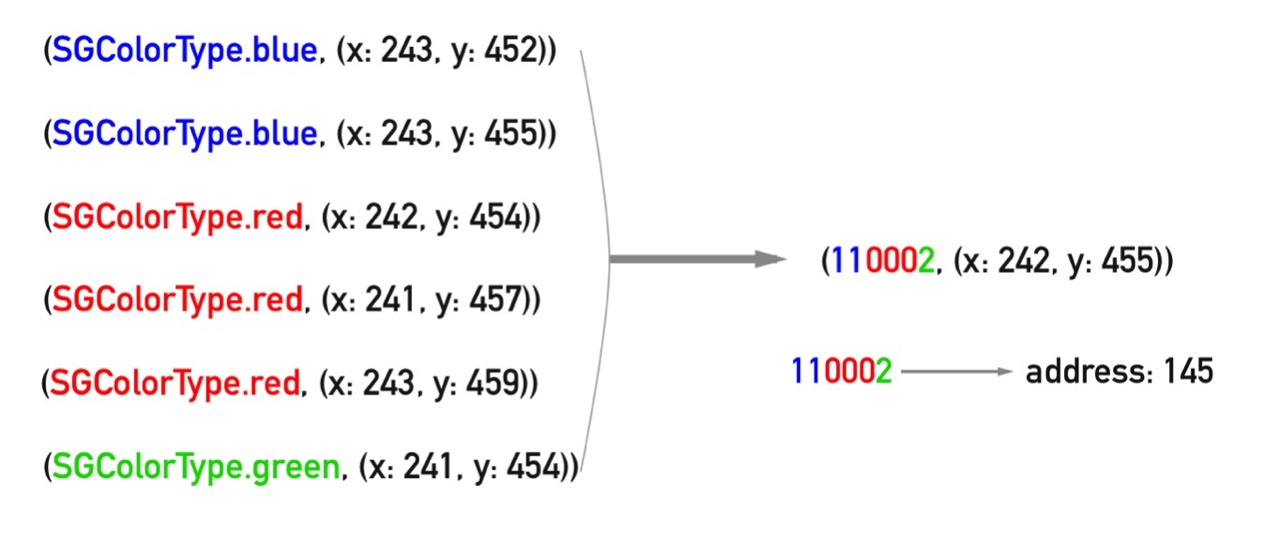
\includegraphics[scale=0.35]{figures/calibration_grouping.jpg}
	\caption{Пример группировки цветов по координатам}
	\label{fig:develop:algorithm:grouping}
\end{figure}

Сопоставление последовательности происходит следующим образом: сперва ищется точка с полностью совпадающей последовательностью цветов, если такой нет, то ищется последовательность отличающаяся на один цвет, потом на два и на три. Далее из всех найденных возможных точек, выбирается ближайшая к остальным уже найденным точкам.

\subsubsection{} Аппроксимация
\label{sec:develop:algorithm:approximation}

После обработки изображения часто остаются нераспознанными некоторые лампочки (обычно 20-30\%). Для устранения данной проблемы используется алгоритм аппроксимации. Он берет соседние найденные лампы возле ненайденных (например 63 и 69 лампочка, если алгоритм не нашел с 64 по 68 лампочку), строит между ними прямую и располагает на равноудаленных участках этого отрезка ненайденные лампочки. Если ненайденные лампочки находятся на концах гирлянды, то он просто строит примерно похожую линию и располагает гирлянды на ней. Это помогает построить примерно похожую гирлянду на экране телефона.

~
\begin{figure}[H]
\centering
	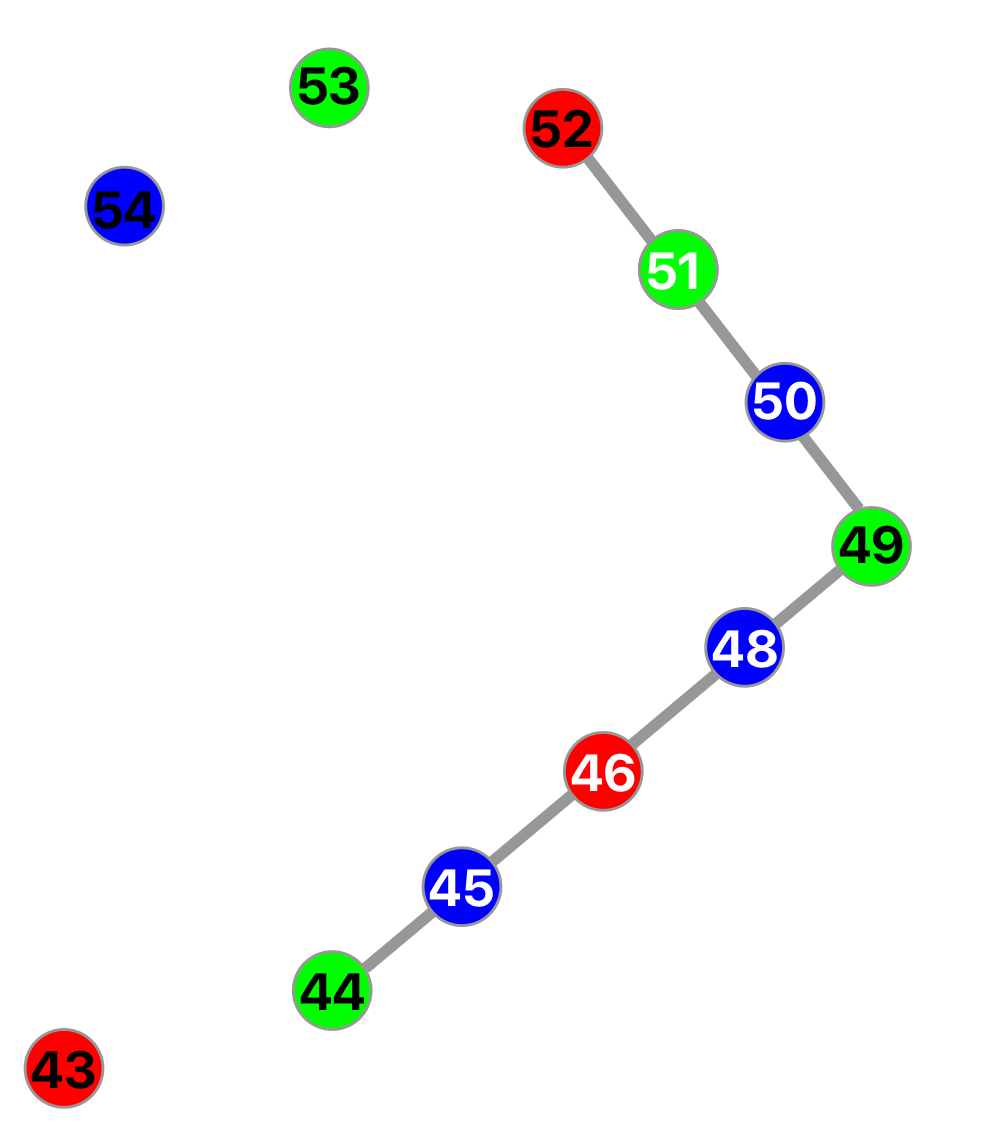
\includegraphics[scale=0.35]{figures/calibration_approximation.png}
	\caption{Пример работы аппроксимации (белым цветом отмечены аппроксимированные лампочки)}
	\label{fig:develop:algorithm:approximation}
\end{figure}